\begin{figure*}[t]
  \centering
  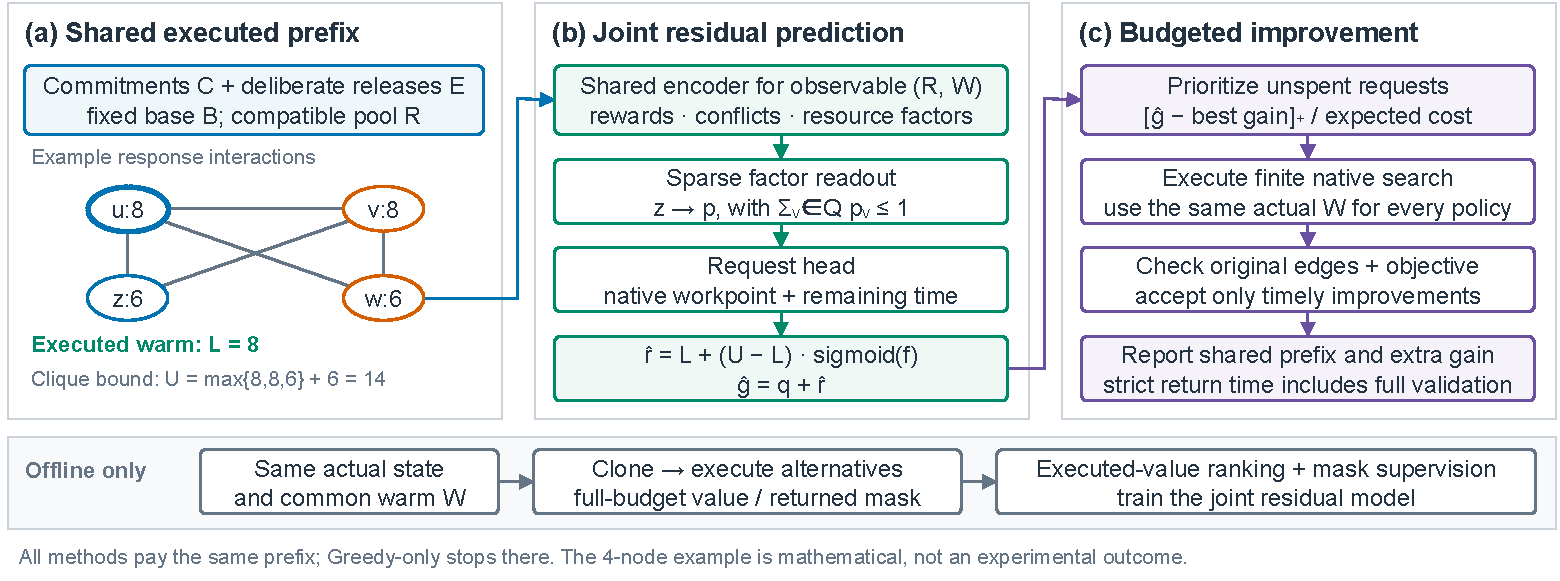
\includegraphics[width=\textwidth]{v4_figures/residual_schematics/method_joint_residual.pdf}
  \caption{Learning additional joint recovery after a common executed greedy
  response. (a) Each commitment/release action determines a fixed base and
  compatible recovery graph. The mathematical four-vertex example has greedy
  value $L=8$, joint optimum $12$, and clique-partition bound $U=14$.
  (b) A shared structural encoder, request-conditioned fractional occupancies,
  and bounded residual head estimate further finite recovery; the known
  immediate gain enters as an exact offset. (c) Predictions prioritize calls
  using the same actual warm membership, while the execution kernel admits
  only validated improvements. Training compares executed alternatives from
  the same snapshot. The example is illustrative, not an empirical result.}
  \label{fig:method-residual}
\end{figure*}
